%============================================================
% MTH 112 Project - Right Triangle Trigonometry
% Updated 202504
%============================================================
% Issue: Include nepal flag
% 2015 Constitution
% The Constitutional Assembly of Nepal adopted 16 November the Constitution of the Federal Democratic Republic of Nepal. In article 8 and Schedule 1 the flag was described.

% Constitution of the Federal Democratic Republic of Nepal
% 8. National flag
% (1) The national flag of Nepal, consists of two juxtaposed triangular figures with a crimson colored base and deep blue borders, there being a white emblem of the crescent moon with eight rays visible out of sixteen in the upper part and a white emblem of a twelve rayed sun in the lower part.
% (2) The method of drawing the flag and other particulars relating thereto shall be as set out in Schedule 1.

% Schedule 1 (Related with clause (2) of Article 8)
% Method of Making the National Flag of Nepal
% (A) Method of Making the shape inside the Border
% (1) On the lower portion of a crimson cloth draw a line AB of the required length from left to right.
% (2) From A draw a line AC perpendicular to AB making AC equal to AB plus one third AB. From AC mark off D making the line AD equal to line AB. Join BD.
% (3) From BD mark off E making BE equal to AB.
% (4) Touching E draw a line FG, starting from the point F on line AC, parallel to AB to the right hand-side. Mark off FG equal to AB.
% (5) Join CG.

% (B) Method of making the Moon
% (6) From AB mark off AH making AH equal to one-fourth of line AB and starting from H draw a line HI parallel to line AC touching line CG at point I.
% (7) Bisect CF at J and draw a line JK parallel to AB touching CG at point K.
% (8) Let L be the point where lines JK and HI cut one another.
% (9) Join JG.
% (10) Let M be the point where line JG and HI cut one another.
% (11) With center M and with a distance shortest from M to BD mark off N on the lower portion of line HI.
% (12) Touching M and starting from O, a point on AC, draw a line from left to right parallel to AB.
% (13) With center L and radius LN draw a semi-circle on the lower portion and let P and Q be the points where it touches the line OM respectively.
% (14) With the center M and radius MQ draw a semi-circle on the lower portion touching P and Q.
% (15) With center N and radius NM draw an arc touching PNQ at R and S. Join RS. Let T be the point where RS and HI cut one another.
% (16) With center T and radius TS draw a semi-circle on the upper portion of PNQ touching at two points.
% (17) With center T and radius TM draw an arc on the upper portion of PNQ touching at two points.
% (18) Eight equal and similar triangles of the moon are to be made in the space lying inside the semi-circle of No (16) and outside the arc of No (17) of his Schedule.

% (C) Method of Making the Sun
% (19) Bisect line AF at U, and draw a line UV parallel to AB line touching line BE at V.
% (20) With center W, the point where HI and UN cut one another and radius MN draw a circle.
% (21) With center W and radius LN draw a circle.
% (22) Twelve equal and similar triangles of the sun are to be made in the space enclosed by the circle of No (20) and No (21) with the two apexes of two triangles touching line HI.

% (D) Method of Making the Border
% (23) The width of the border will be equal to the width of TN. This will be of deep blue color and will be provided on all the sides of the flag. However, on the given angles of the flag the external angles will be equal to the internal angles.
% (24) The above mentioned border will be provided if the flag is to be used with a rope. On the other hand, if it is to be hoisted on a pole, the hole on the border on the side AC can be extended according to requirements.
% Explanation:- The lines HI, RS, FE, ED, JG, OQ, JK and UV are imaginary. Similarly, the external and internal circles of the sun and the other arcs except the crescent moon are imaginary. These are not shown on the flag.



\section{Right Triangle Trigonometry} \label{section-right-triangle-trigonometry}
In this section we will use right triangles to evaluate trigonometric functions, find function values for $\ang{30}$, $\ang{45}$, and $\ang{60}$, use all six trigonometric functions to find lengths inside right triangles, and use right-triangle trigonometry to solve applied problems.

\textbook{\href{https://openstax.org/books/algebra-and-trigonometry-2e/pages/7-2-right-triangle-trigonometry}{7.2}}

\subsection*{Preparation Exercises} \label{preparation-exercises-section-right-triangle-trigonometry}

Answer the following without using a calculator. These questions are intended to check the prerequisite skills needed to complete the rest of the lab.

\begin{myPrep}
	What does the word \say{adjacent} mean?
	\vfill
\end{myPrep}

\begin{myPrep}
	Fill in the table with the missing angle measurements.
			\begin{center}
			\renewcommand{\arraystretch}{1.5} 
				\begin{tabular}{|| c | P{1cm} | P{1cm} | P{1cm} | P{1cm} | P{1cm} | P{1cm} | P{1cm} | P{1cm} ||}
					\hline
					Angle (radians) & $\frac{\pi}{4}$ &  &  & $\frac{2\pi}{3}$ & $\frac{5\pi}{6}$ &  & $\pi$ &  \\
					\hline
					Angle (degrees) &  & $\ang{30}$ & $\ang{90}$ &  &  & $\ang{60}$ &  & $\ang{135}$ \\ 
					\hline
				\end{tabular}
			\end{center}
			\vfill
\end{myPrep}

\begin{myPrep}
	\parbox[t]{0.6\linewidth}{
					Recall that \say{similar triangles} are two triangles with equal angle measurements, but not necessarily equal side lengths. The ratio of any two corresponding sides of the triangles will be equal, which means that $\frac{A_1}{b_1}=\frac{A_2}{b_2}=\frac{A_3}{b_3}$.
					}
						\raisebox{-\height}{
						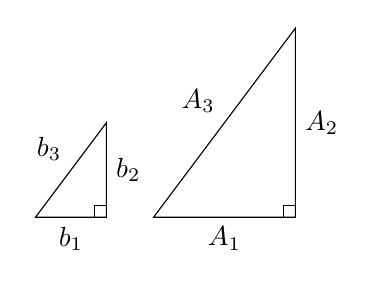
\begin{tikzpicture}[scale=0.3]
							\draw   (0,0)--(1.5,0) coordinate[label=below:$b_1$]--
        							(3,0)--(3,2) coordinate[label=right:$b_2$]--
        							(3,4)--(1.5,2) coordinate[label=above left:$b_3$]--cycle;
        					
        					\draw   (5,0)--(8,0) coordinate[label=below:$A_1$]--
        							(11,0)--(11,4) coordinate[label=right:$A_2$]--
        							(11,8)--(8,4) coordinate[label=above left:$A_3$]--cycle;
        					
        					\draw   (2.5,0)--(2.5,.5)--(3,.5)--(3,0)--cycle;
        					\draw  	(11,0)--(11,.5)--(10.5,.5)--(10.5,0)--cycle;
						\end{tikzpicture}
						}

				\parbox[t]{0.6\linewidth}{
					Using the similar triangles equations, solve for the missing sides. Drawing may not be drawn to scale.
					}
						\raisebox{-\height}{
						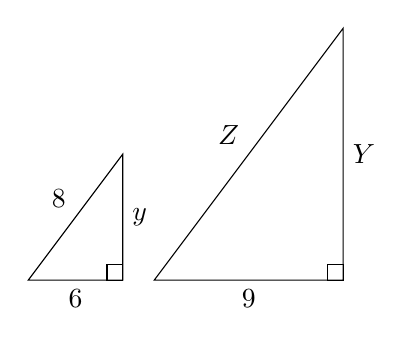
\begin{tikzpicture}[scale=0.4]
							\draw   (0,0)--(1.5,0) coordinate[label=below:$6$]--
        							(3,0)--(3,2) coordinate[label=right:$y$]--
        							(3,4)--(1.5,2) coordinate[label=above left:$8$]--cycle;
        					\draw   (4,0)--(7,0) coordinate[label=below:$9$]--
        							(10,0)--(10,4) coordinate[label=right:$Y$]--
        							(10,8)--(7,4) coordinate[label=above left:$Z$]--cycle;
        					\draw   (2.5,0)--(2.5,.5)--(3,.5)--(3,0)--cycle;
        					\draw  	(10,0)--(10,.5)--(9.5,.5)--(9.5,0)--cycle;
						\end{tikzpicture}
						}
\end{myPrep}
\vfill

%======================================================
\newpage
%======================================================

\subsection*{Practice Exercises} \label{practice-exercises-section-right-triangle-trigonometry}

\begin{myPractice}
	Decide which values match without a calculator using \say{SOHCAHTOA} and \say{CHOSHACAO}. The triangles are not shown to scale.
		\begin{enumerate}
			\begin{multicols}{2}
				\item Which of the values will be the same as $\sin(\ang{40})$?
					\begin{itemize}
						\item $\sin(\ang{50})$
						\item $\cos(\ang{50})$
						\item $\tan(\ang{40})$
						\item $\cos(\ang{40})$
					\end{itemize}
				\columnbreak
					\begin{center}\captionsetup{type=figure} \captionof{figure}{A right triangle}
						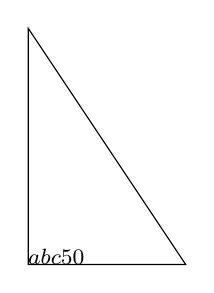
\begin{tikzpicture}[thin] \label{section-right-triangle-trig-example-triangle}
							\coordinate (O) at (0,0);
							\coordinate (A) at (2,0);
							\coordinate (B) at (0,3);
							\draw (O)--(A)--(B)--cycle;
							\footnotesize
							\tkzLabelSegment[below=2pt](O,A){$a$}
							\tkzLabelSegment[left=2pt](O,B){$b$}
							\tkzLabelSegment[above=2pt, rotate=-atan(3/2)](A,B){$c$}
							\tkzMarkRightAngle[size=0.5](A,O,B)
							\tkzMarkAngle[size=0.9cm](B,A,O)
							\tkzLabelAngle[pos = 0.6](B,A,O){$\ang{50}$}
							\tkzMarkAngle[size=0.7cm](O,B,A)
							% \tkzLabelAngle[pos = 0.5](O,B,A){$\beta$}
						\end{tikzpicture}
					\end{center}
				\end{multicols}

			\begin{multicols}{2}
				\item Which of the values will be the same as $\tan(\ang{20})$?
					\begin{itemize}
						\item $\cot(\ang{20})$
						\item $\tan(\ang{70})$
						\item $\cot(\ang{70})$
						\item $\cos(\ang{70})$
					\end{itemize}
				\columnbreak
					\begin{center}\captionsetup{type=figure} \captionof{figure}{A right triangle}
						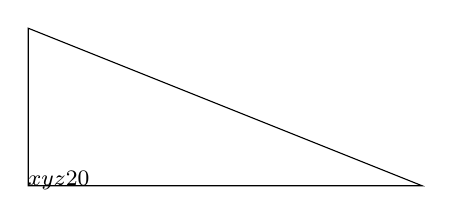
\begin{tikzpicture}[thin] \label{section-right-triangle-trig-example-triangle2}
							\coordinate (O) at (0,0);
							\coordinate (A) at (5,0);
							\coordinate (B) at (0,2);
							\draw (O)--(A)--(B)--cycle;
							\footnotesize
							\tkzLabelSegment[below=2pt](O,A){$x$}
							\tkzLabelSegment[left=2pt](O,B){$y$}
							\tkzLabelSegment[above=2pt, rotate=-atan(2/5)](A,B){$z$}
							\tkzMarkRightAngle[size=0.5](A,O,B)
							\tkzMarkAngle[size=1.3cm](B,A,O)
							\tkzLabelAngle[pos = 1](B,A,O){$\ang{20}$}
							\tkzMarkAngle[size=0.7cm](O,B,A)
							% \tkzLabelAngle[pos = 0.5](O,B,A){$\beta$}
						\end{tikzpicture}
					\end{center}
				\end{multicols}
		\end{enumerate}
\end{myPractice}

\begin{myPractice}
	\begin{multicols}{2}
		For the triangle shown in Figure \ref{section-right-triangle-trig-example-triangle-solving2}, find $a$, $c$, and $\alpha$. You can use a calculator to help get an approximation, accurate to 4 digits behind the decimal place.
		\columnbreak
		\begin{center}\captionsetup{type=figure}\captionof{figure}{A right triangle}
			\begin{tikzpicture}[thin] \label{section-right-triangle-trig-example-triangle-solving2}
				\coordinate (O) at (0,0);
				\coordinate (A) at (7,0);
				\coordinate (B) at (0,3);
				\draw (O)--(A)--(B)--cycle;
				\footnotesize
				\tkzLabelSegment[below=2pt](O,A){$a$}
				\tkzLabelSegment[left=2pt](O,B){$28\text{m}$}
				\tkzLabelSegment[above right=2pt](A,B){$c$}
				\tkzMarkRightAngle[size=0.5](A,O,B)
				\tkzMarkAngle[size=0.8cm](B,A,O)
				\tkzLabelAngle[pos = 0.6](B,A,O){$\alpha$}
				\tkzMarkAngle[size=0.7cm](O,B,A)
				\tkzLabelAngle[pos = 0.5](O,B,A){$\ang{58}$}
			\end{tikzpicture}
		\end{center}
	\end{multicols}
\end{myPractice}
\vfill
\vfill

%======================================================
\newpage
%======================================================

\begin{myPractice}
	On a backpacking trip in the Wallowa Mountains of northeastern Oregon, Megan and Emily were marveling at the height of an enormous Ponderosa Pine. Ross said, \say{we can calculate it's height pretty easily just by knowing that \say{a pace} is $3\text{ft}$ and the distance from the tip of my thumb to the tip of my pinkie is $9$ inches}. Ross paced away from the tree on level ground $30$ paces. Help the three hikers measure the height of the tree two different ways.
	\begin{enumerate}
		\begin{multicols}{2}
			\item Ross finds a stick and measures it to be about $6\text{ft}$ tall. He lays down on the ground and asks Emily to hold the stick vertically on the ground at a certain point where the tip of the stick lines up with the tip of the tree from his point of view. That distance on the ground was $4\text{ft}$ from Ross's viewing position, as shown in Figure \ref{figure-right-triangle-trig-practice-tree-1}. Set up similar triangles to estimate the height of the tree. Drawing not to scale.
			\begin{center}
				\begin{tikzpicture}
					\begin{axis}[
						axis x line=none,
						axis y line=none,
						xlabel=none,
						ylabel=none,
						xmin=-5,xmax=110,
						ymin=-5,ymax=140,
						clip=false,
						]	
							\node   [inner sep=0pt] (Ponderosa) at (88,67) {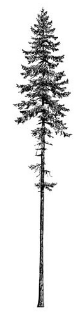
\includegraphics[width=.069\textwidth]{Ponderosalookalike.png}};
							\draw   [color=second,thin](0,0)--(90,0)--(90,135)--cycle;
							\draw   [color=second,thin](83,0)--(83,8)--(90,8);
							\draw   [thin,color=third](0,-10)--(0,-15)--(90,-15)--(90,-10);
							\draw   [color=third](45,-15) coordinate[label=below:$90$ft];

							\draw   [thin,color=first](5.4,0)--(5.4,3)--(8,3);
							\draw   [thin,color=fourth](0,-1)--(0,-2)--(8,-2)--(8,-1);
							\draw   [color=fourth](4,-1) coordinate[label=below:\tiny{$4$ft}];

        					\draw   [very thick,color=first](8,0)--(8,12);
        					\draw   [thin,color=first](10,1)--(11,1)--(11,12)--(10,12);
							\draw   [color=first](10,7) coordinate[label=right:\footnotesize{$6$ft stick}];
					\end{axis}
				\end{tikzpicture}
			\end{center}\captionsetup{type=figure}\captionof{figure}{A tree in the woods}\label{figure-right-triangle-trig-practice-tree-1}
		\end{multicols}
		\vfill

		\begin{multicols}{2}
			\item Ross then took out his phone and used the inclinometer app on to measure the angle to to top of the tree, to be about $\ang{55}$. In this scenario, Ross still $30$ paces away from the tree, and was standing to measure the height: the phone was $5\text{ft}$ above the ground, as shown in Figure \ref{figure-right-triangle-trig-practice-tree-2}. Use right-triangle trigonometry to estimate the height of the tree. Drawing not to scale.
			\begin{center}
				\begin{tikzpicture}
					\begin{axis}[
						axis x line=none,
						axis y line=none,
						xlabel=none,
						ylabel=none,
						xmin=-5,xmax=110,
						ymin=-5,ymax=140,
						clip=false,
						]
							\node   [inner sep=0pt] (Ponderosa) at (88,67) {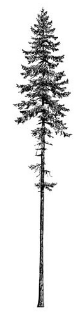
\includegraphics[width=.069\textwidth]{Ponderosalookalike.png}};
							\draw   [thin,color=second](0,0)--(90,0)--(90,135)--(0,10)--cycle;
							\draw   [color=second,thin](83,0)--(83,8)--(90,8);
							\draw   [color=first](-1,5) coordinate[label=left:\footnotesize{$5$ft}];
        					\draw   [thin,color=first](-2,0)--(-3,0)--(-3,10)--(-2,10);
							\draw   [color=third](45,-10) coordinate[label=below:$90$ft];
							\draw   [thin,color=third](0,-5)--(0,-10)--(90,-10)--(90,-5);
							\draw   [color=fourth](10,16)coordinate[label=right:\footnotesize$\ang{55}$];
							\draw   [thin,dashed,color=fourth] (90,10)--(0,10);
        					\addplot[variable=\t, domain=0:55, samples=50,very thin, color=fourth]({8*cos(t)}, {8*sin(t)+10});  
					\end{axis}
				\end{tikzpicture}
			\end{center}\captionsetup{type=figure}\captionof{figure}{A tree in the woods}\label{figure-right-triangle-trig-practice-tree-2}
		\end{multicols}
		\vfill
	\end{enumerate}
\end{myPractice}

%======================================================
\newpage
%======================================================

\subsection*{Definitions} \label{definitions-section-right-triangle-trig}

Consider the triangle shown in Figure \ref{section-right-triangle-trig-definitions}.
		\begin{center}
			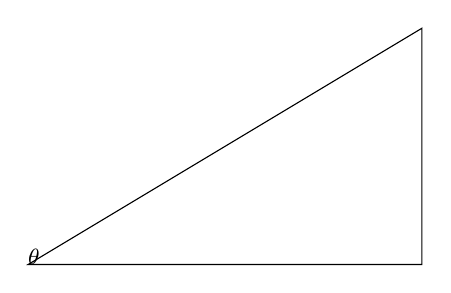
\begin{tikzpicture}[thin]
				\coordinate (O) at (0,0);
				\coordinate (A) at (5,0);
				\coordinate (B) at (5,3);
				\draw (O)--(A)--(B)--cycle;
				\footnotesize
				\tkzLabelSegment[below=2pt](O,A){Adjacent}
				\tkzLabelSegment[above=2pt,rotate=atan(3/5)](O,B){Hypotenuse}
				\tkzLabelSegment[above=2pt,rotate=-90](A,B){Opposite}

				\tkzMarkRightAngle[size=0.5](O,A,B)
				% \tkzMarkAngle[size=0.8cm](O,B,A)
				% \tkzLabelAngle[pos = 0.6](O,B,A)
				\tkzMarkAngle[size=0.9cm](A,O,B)
				\tkzLabelAngle[pos = 0.7](A,O,B){$\theta$}
			\end{tikzpicture}\captionsetup{type=figure}\captionof{figure}{A right triangle}\label{section-right-triangle-trig-definitions}
		\end{center}

\begin{myDefinition}[{SOHCAHTOA}]~\\[0.5mm]
	\say{SOHCAHTOA} stands for 
	\begin{itemize}
		\item \textbf{S}ine is \textbf{O}pposite over \textbf{H}ypotenuse
		\item \textbf{C}osine is \textbf{A}djacent over \textbf{H}ypotenuse
		\item \textbf{T}angent is \textbf{O}pposite over \textbf{A}djacent
	\end{itemize}

	These mean the following:

	\begin{itemize}
		\begin{multicols}{3}
			\item  $\sin(\theta)=\frac{\text{Opposite}}{\text{Hypotenuse}}$
			\item  $\cos(\theta)=\frac{\text{Adjacent}}{\text{Hypotenuse}}$
			\item  $\tan(\theta)=\frac{\text{Opposite}}{\text{Adjacent}}$
		\end{multicols}
	\end{itemize}
\end{myDefinition}

\vfill
\begin{myDefinition}[{CHOSHACAO}]~\\[0.5mm]
	\label{CHOSHACAO}
	\say{CHOSHACAO} stands for 
	\begin{itemize}
		\item \textbf{C}osecant is \textbf{H}ypotenuse over \textbf{O}pposite
		\item \textbf{S}ecant is \textbf{H}ypotenuse over \textbf{A}djacent
		\item \textbf{C}otangent is \textbf{A}djacent over \textbf{O}pposite
	\end{itemize}

	These mean the following:

	\begin{itemize}
		\begin{multicols}{3}
			\item  $\csc(\theta)=\frac{\text{Hypotenuse}}{\text{Opposite}}$
			\item  $\sec(\theta)=\frac{\text{Hypotenuse}}{\text{Adjacent}}$
			\item  $\cot(\theta)=\frac{\text{Adjacent}}{\text{Opposite}}$
		\end{multicols}
	\end{itemize}
\end{myDefinition}
\vfill
%======================================================
\newpage
%======================================================

\subsection*{Exit Exercises} \label{exit-exercises-section-right-triangle-trigonometry}

\begin{myExit}
Use the triangle in Figure \ref{figure-right-triangle-trig-exit-triangle} to answer the questions below.
	\begin{center}
		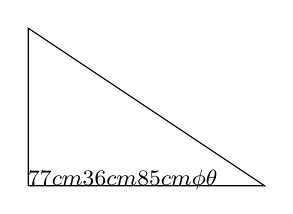
\begin{tikzpicture}[thin]
		%36, 77, 85
			\coordinate (O) at (0,0);
			\coordinate (A) at (3,0);
			\coordinate (B) at (0,2);
			\draw (O)--(A)--(B)--cycle;
			\footnotesize
			\tkzLabelSegment[below=2pt](O,A){$77\text{cm}$}
			\tkzLabelSegment[above=2pt,rotate=90](O,B){$36\text{cm}$}
			\tkzLabelSegment[above=2pt,rotate=-atan(2/3)](A,B){$85\text{cm}$}
			\tkzMarkRightAngle[size=0.5](A,O,B)
			\tkzMarkAngle[size=0.8cm](B,A,O)
			\tkzLabelAngle[pos = 0.6](B,A,O){$\phi$}
			\tkzMarkAngle[size=0.7cm](O,B,A)
			\tkzLabelAngle[pos = 0.5](O,B,A){$\theta$}
		\end{tikzpicture}
	\end{center}\captionsetup{type=figure} \captionof{figure}{A right triangle}\label{figure-right-triangle-trig-exit-triangle}
	\begin{enumerate}[label=(\roman*)]
		\begin{multicols}{3}
			\item Find the value of $\cos(\theta)$.
			\item Find the value of $\tan(\phi)$.
			\item Find the value of $\csc(\theta)$.
		\end{multicols}
	\end{enumerate}
\end{myExit}
\vfill

\begin{myExit}
	Shown in Figure \ref{figure-right-triangle-trig-exit-triangle-SOHCAHTOA} is a triangle with side $b=11$, angle $B=\ang{22}$, and angle $C=\ang{90}$. Find the length of the side $a$.
		\begin{center}
			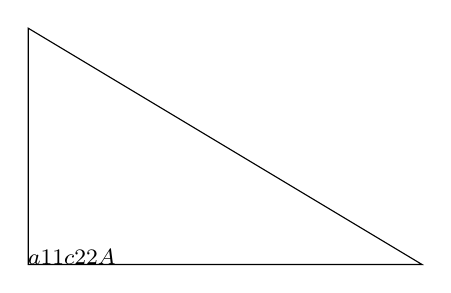
\begin{tikzpicture}[thin] 
				\coordinate (O) at (0,0);
				\coordinate (A) at (5,0);
				\coordinate (B) at (0,3);
				\draw (O)--(A)--(B)--cycle;
				\footnotesize
				\tkzLabelSegment[below=2pt](O,A){$a$}
				\tkzLabelSegment[left=2pt](O,B){$11$}
				\tkzLabelSegment[above right=2pt](A,B){$c$}
				\tkzMarkRightAngle[size=0.5](A,O,B)
				\tkzMarkAngle[size=1.2cm](B,A,O)
				\tkzLabelAngle[pos = 0.6, left](B,A,O){\footnotesize$\ang{22}$}
				\tkzMarkAngle[size=0.7cm](O,B,A)
				\tkzLabelAngle[pos = 0.5](O,B,A){$A$}
			\end{tikzpicture}
		\end{center}\captionsetup{type=figure}\captionof{figure}{A right triangle}\label{figure-right-triangle-trig-exit-triangle-SOHCAHTOA}
\end{myExit}
\vfill
\exitlikert{right triangle trigonometry}